\documentclass[a4paper,12pt,twoside,openany]{report}
%
% Wzorzec pracy dyplomowej
% J. Starzynski (jstar@iem.pw.edu.pl) na podstawie pracy dyplomowej
% mgr. inż. Błażeja Wincenciaka
% Wersja 0.1 - 8 października 2016
%
\usepackage{polski}
\usepackage{helvet}
\usepackage[T1]{fontenc}
\usepackage{anyfontsize}
\usepackage[utf8]{inputenc}
\usepackage[pdftex]{graphicx}
\usepackage{tabularx}
\usepackage{array}
\usepackage{listings}
\usepackage[polish]{babel}
\usepackage{subfigure}
\usepackage{amsfonts}
\usepackage{verbatim}
\usepackage{indentfirst}
\usepackage[pdftex]{hyperref}


% rozmaite polecenia pomocnicze
% gdzie rysunki?
\newcommand{\ImgPath}{.}

% oznaczenie rzeczy do zrobienia/poprawienia
\newcommand{\TODO}{\textbf{TODO}}


% wyroznienie slow kluczowych
\newcommand{\tech}{\texttt}

% na oprawe (1.0cm - 0.7cm)*2 = 0.6cm
% na oprawe (1.1cm - 0.7cm)*2 = 0.8cm
%  oddsidemargin lewy margines na nieparzystych stronach
% evensidemargin lewy margines na parzystych stronach
\def\oprawa{1.05cm}
\addtolength{\oddsidemargin}{\oprawa}
\addtolength{\evensidemargin}{-\oprawa}

% table span multirows
\usepackage{multirow}
\usepackage{enumitem}	% enumitem.pdf
\setlist{listparindent=\parindent, parsep=\parskip} % potrzebuje enumitem

%%%%%%%%%%%%%%% Dodatkowe Pakiety %%%%%%%%%%%%%%%%%
\usepackage{prmag2017}   % definiuje komendy opieku,nrindeksu, rodzaj pracy, ...


%%%%%%%%%%%%%%% Strona Tytułowa %%%%%%%%%%%%%%%%%
% To trzeba wypelnic swoimi danymi
\title{Wykorzystanie protokołu HTTP/2 do budowy szybkiej aplikacji internetowej}

% autor
\author{Piotr Szklanko}
\nrindeksu{244145}

\opiekun{mgr inż. Bartosz Chaber}
\terminwykonania{1 lutego 2017} % data na oświadczeniu o samodzielności
\rok{2017}


% Podziekowanie - opcjonalne
% \podziekowania{\noindent
{\Large Podziękowania}
\bigskip

Dziękujemy bardzo serdecznie wszystkim, a w szczególności Rodzinom i~Unii Europejskiej...

\bigskip

{\raggedleft
Zdolny Student i Pracowity Kolega

}

}

% To sa domyslne wartosci
% - mozna je zmienic, jesli praca jest pisana gdzie indziej niz w ZETiIS
% - mozna je wyrzucic jesli praca jest pisana w ZETiIS
%\miasto{Warszawa}
%\uczelnia{POLITECHNIKA WARSZAWSKA}
%\wydzial{WYDZIAŁ ELEKTRYCZNY}
%\instytut{INSTYTUT ELEKTROTECHNIKI TEORETYCZNEJ\linebreak[1] I~SYSTEMÓW INFORMACYJNO-POMIAROWYCH}
% \zaklad{ZAKŁAD ELEKTROTECHNIKI TEORETYCZNEJ\linebreak[1] I~INFORMATYKI STOSOWANEJ}
\rodzajpracy{INŻYNIERSKA}
%\kierunekstudiow{INFORMATYKA}
%%% koniec od P.W

\opinie{%
  \newpage
\begin{center}
 {\large\bf  Opinia} \\
o pracy dyplomowej magisterskiej wykonanej przez dyplomanta\\
{\bf Zdolnego Studenta i Pracowitego Kolegę} \\
 Wydział Elektryczny, kierunek Informatyka,  Politechnika Warszawska\\
Temat pracy\\
\textit{\bf
TYTUŁ PRACY DYPLOMOWEJ
}\\
\end{center}
\medskip
\noindent
Promotor: {\bf dr inż. Miły Opiekun}\\
Ocena pracy dyplomowej: {\bf bardzo dobry}

\medskip

\centerline{\bf Treść opinii}
   Celem pracy dyplomowej panów dolnego Studenta i Pracowitego Kolegi  było
opracowanie systemu pozwalającego symulować  i opartego o oprogramowanie o
otwartych źródłach (ang. Open Source). Jak piszą Dyplomanci, starali się opracować
system, który łatwo będzie dostosować do zmieniających się dynamicznie wymagań,
będzie miał niewielkie wymagania sprzętowe i umożliwiał dalszą łatwą rozbudowę oraz
dostosowanie go do potrzeb.
Przedstawiona do recenzji praca składa się z krótkiego wstępu jasno i
wyczerpująco opisującego oraz uzasadniającego cel pracy, trzech rozdziałów (2-4)
zawierających opis istniejących podobnych
rozwiązań, komponentów rozpatrywanychjako kandydaci do
tworzonego systemu i wreszcie zagadnień wydajności wirtualnych
rozwiązań. Piąty rozdział to opis przygotowanego przez
Dyplomantów środowiska obejmujący opis konfiguracji
środowiska oraz przykładowe ćwiczenia laboratoryjne. Ostatni
rozdział pracy to opis możliwości dalszego
rozwoju projektu. W ramach przygotowania pracy Dyplomanci zebrali i przedstawili w
bardzo przejrzysty sposób duży zasób informacji, co świadczy o dobrej orientacji
w nowoczesnej i ciągle intensywnie rozwijanej tematyce stanowiącej
zakres pracy i o umiejętności przejrzystego przedstawienia tych
wyników. Praca zawiera dwa dodatki, z których pierwszy obejmuje wyniki
eksperymentów i badań nad wydajnością, a drugi to źródła
skryptów budujących środowisko.

 Dyplomanci dość
dobrze zrealizowali postawione przed nimi zadanie,
wykazali się więc umiejętnością zastosowania w praktyce wiedzy
przedstawionej w rozdziałach 2-4.  Uważam, że cele postawione w założeniach pracy zostały pomyślnie
zrealizowane. Proponuję ocenę bardzo dobrą (5).

\vskip 1cm
{
\raggedleft
(data, podpis)\kern1cm

}
  \newpage
  \newpage
\begin{center}
 {\large\bf  Recenzja } \\
pracy dyplomowej magisterskiej wykonanej przez dyplomanta\\
{\bf Zdolnego Studenta i Pracowitego Kolegę} \\
 Wydział Elektryczny, kierunek Informatyka,  Politechnika Warszawska\\
Temat pracy\\
\textit{\bf
TYTUŁ PRACY DYPLOMOWEJ
}\\
\end{center}
\medskip
\noindent
Recenzent: {\bf prof. nzw. dr hab. inż. Jan Surowy}\\
Ocena pracy dyplomowej: {\bf bardzo dobry}
\medskip


\centerline{\bf Treść recenzji}
   Celem pracy dyplomowej panów dolnego Studenta i Pracowitego Kolegi  było
opracowanie systemu pozwalającego symulować  i opartego o oprogramowanie o
otwartych źródłach (ang. Open Source). Jak piszą Dyplomanci, starali się opracować
system, który łatwo będzie dostosować do zmieniających się dynamicznie wymagań,
będzie miał niewielkie wymagania sprzętowe i umożliwiał dalszą łatwą rozbudowę oraz
dostosowanie go do potrzeb.
Przedstawiona do recenzji praca składa się z krótkiego wstępu jasno i
wyczerpująco opisującego oraz uzasadniającego cel pracy, trzech rozdziałów (2-4)
zawierających bardzo solidny i przejrzysty opis: istniejących podobnych
rozwiązań (rozdz. 2), komponentów rozpatrywanychjako kandydaci do
tworzonego systemu (rozdz. 3) i wreszcie zagadnień wydajności wirtualnych
rozwiązań, zwłaszcza w kontekście współpracy  kilku elementów
 sieci (rozdział 4). Piąty rozdział to opis przygotowanego przez
Dyplomantów środowiska obejmujący opis konfiguracji
środowiska oraz przykładowe ćwiczenia laboratoryjne (5 ćwiczeń). Ostatni, szósty
rozdział pracy to krótkie zakończenie, które wylicza także możliwości dalszego
rozwoju projektu. W ramach przygotowania pracy Dyplomanci zebrali i przedstawili w
bardzo przejrzysty sposób duży zasób informacji o narzędziach, Rozdziały 2, 3 i 4 świadczą o dobrej orientacji
w nowoczesnej i ciągle intensywnie rozwijanej tematyce stanowiącej
zakres pracy i o umiejętności syntetycznego, przejrzystego przedstawienia tych
wyników. Drobne  mankamenty tej części pracy to zbyt skrótowe omawianie
niektórych zagadnień technicznych, zakładające dużą początkową wiedzę czytelnika
i dość niestaranne podejście do powołań na źródła.
Utrudnia to w pewnym stopniu czytanie pracy i zmniejsza jej wartość dydaktyczną
(a ta zdaje się być jednym z celów Autorów), ale jest zrekompensowane zawartością
merytoryczną. Praca zawiera dwa dodatki, z których pierwszy obejmuje wyniki
eksperymentów i badań nad wydajnością, a drugi to źródła
skryptów budujących środowisko. Praca
zawiera niestety dość dużą liczbę drobnych błędów redakcyjnych, ale nie wpływają
one w sposób istotny na na jej czytelność i wartość. W całej pracy przewijają
się samodzielne, zdecydowane wnioski Autorów, które są wynikiem własnych i
oryginalnych badań.  Rozdział 5 i dodatki pracy przekonują mnie, że Dyplomanci dość
dobrze zrealizowali postawione przed nimi zadanie. Pozwala to stwierdzić, że
wykazali się więc także umiejętnością zastosowania w praktyce wiedzy
przedstawionej w rozdziałach 2-4. Kończący pracę rozdział szósty świadczy o
dużym (ale moim zdaniem uzasadnionym) poczuciu własnej wartości i jest
świadectwem własnego, oryginalnego spojrzenia na tematykę przedstawioną w pracy
dyplomowej. Uważam, że cele postawione w założeniach pracy zostały pomyślnie
zrealizowane. Proponuję ocenę bardzo dobrą (5).

\vskip 1cm
{
\raggedleft
(data, podpis)\kern1cm

}
}

\streszczenia{
  \newpage
\begin{center}
\large \bf
Wykorzystanie protokołu HTTP/2.0 do budowy szybkiej aplikacji internetowej
\end{center}

\section*{Streszczenie}
Praca składa się z krótkiego wstępu jasno i
wyczerpująco opisującego oraz uzasadniającego cel pracy, trzech rozdziałów (2-4)
zawierających opis istniejących podobnych
rozwiązań, komponentów rozpatrywanychjako kandydaci do
tworzonego systemu i wreszcie zagadnień wydajności wirtualnych
rozwiązań. Piąty rozdział to opis  środowiska obejmujący opis konfiguracji
środowiska oraz przykładowe ćwiczenia laboratoryjne. Ostatni
rozdział pracy to opis możliwości dalszego
rozwoju projektu. 

\bigskip
{\noindent\bf Słowa kluczowe:} praca dyplomowa, LaTeX, jakość

\vskip 2cm


\begin{center}
\large \bf
THESIS TITLE
\end{center}

\section*{Abstract}
This thesis presents a novel way of using a novel algorithm to solve complex
problems of filter design. In the first chapter the fundamentals of filter design
are presented. The second chapter describes an original algorithm invented by the
authors. Is is based on evolution strategy, but uses an original method of filter
description similar to artificial neural network. In the third chapter the implementation
of the algorithm in C programming language is presented. The fifth chapter contains results
of tests which prove high efficiency and enormous accuracy of the program. Finally some
posibilities of further development of the invented algoriths are proposed.

\bigskip
{\noindent\bf Keywords:} thesis, LaTeX, quality

\vfill
}

\begin{document}
\maketitle

%-----------------
% Wstęp
%-----------------
\chapter{Wstęp}
Moim celem jest przeprowadzenie testów protokołu HTTP w najnowszej wersji 2.0.
Obecnie powszechnie stosowana jest wersja 1.1, która została wprowadzona w roku 1999.
Jednakże szybki rozwój technologii internetowych sprawia, że wprowadzony osiemnaście lat temu protokół przestaje powoli spełniać swoje zadanie.
Obecnie bez wykorzystania serwerów CDN czy cache przeglądarki oraz innych sposobów nie jest możliwe stworzenie płynnie działającej strony internetowej.
Za pomocą własnoręcznie stworzonej aplikacji chcę przekonać się, czy wprowadzone funkcje faktycznie mają tak ogromny wpływ na szybkość komunikacji pomiędzy klientem i serwerem.

Swoją aplikację stworzyłem wykorzystując zestaw oprogramowania MEAN -- MongoDB, Express.js, Angular i Node.js.
\begin{itemize}
	\item MongoDB -- baza danych NoSQL (cos o mongoose? dodać dokumentację do wszystkich punktów),
	\item Express.js -- framework Node.js do tworzenia aplikacji sieciowych od strony serwera,
	\item Angular -- framework JavaScript służący do budowy dynamicznej aplikacji internetowej od strony użytkownika,
	\item Node.js -- środowisko uruchumieniowe języka JavaScript, które pozwala wystartować serwer.
\end{itemize}
Zdecydowałem się na to rozwiązanie z kilku powodów:
\begin{itemize}
	\item po przejrzeniu dostępnych w sieci informacji doszedłem do wniosku, że implementacja protokołu HTTP/2 jest najlepiej opisana oraz wspierana przez środowisko związane z JavaScriptem,
	\item dobra znajomość języka JavaScript oraz jednoczesna chęć rozwoju umiejętności tworzenia aplikacji w tym języku,
	\item chęć poszerzenia wiedzy dotyczącej budowania aplikacji internetowych za pomocą technologii javascriptowych,
	\item nie ukrywam, że znaczący wpływ na moją decyzję miała również popularność języka JavaScript na rynku pracy.
\end{itemize}

%-----------------
% HTTP/2.0
%-----------------
\chapter{HTTP/2}

\section{Historia}
\label{sectionHistoria}
Pracę nad zmianami w protokole zapoczątkowała w 2009 roku firma Google ze swoim projektem SPDY.
Zdecydowali się oni na stworzenie protokołu, który miał usprawnić działanie aplikacji oraz stron internetowych rozwiązując ograniczenia nałożone przez HTTP/1.1.
Z biegiem czasu coraz więcej przeglądarek oraz stron internetowych, zarówno tych dużych jak i tych małych, zaczęło wspierać SPDY, co zainteresowało osoby pracujące nad protokołem HTTP.
Zdecydowali się oni wykorzystać dokumentację protokołu SPDY jako początek prac nad własnym protokołem -- HTTP/2.
Od tego momentu aż do roku 2015, kiedy to standard HTTP/2 został oficjalnie zaakceptowany 
(\TODO odnośnik RFC 7540 i może 7541), projekty były rozwijane równolegle.
SPDY było wykorzystywane do testów nowych funkcjonalności, które miały zostać wprowadzone do nowego protokołu HTTP.
Niedługo po oficjalnym zaakceptowaniu HTTP/2 ogłoszono, że SPDY nie będzie dalej wspierane.

W kilku poniższych akapitach postaram się przybliżyć zmiany, które zostały wprowadzone do protokołu HTTP.

\section{Protokół binarny}
\label{sectionProtokolBinarny}

Kluczową zmianą, która determinuje brak wstecznej kompatybilności z HTTP/1.1, jest przejście na kodowanie binarne przesyłanych wiadomości. Przykładowa ramka widoczna jest na rysunku \ref{schematRamki}
\begin{figure}[!htbp]
	\begin{center}
\centering
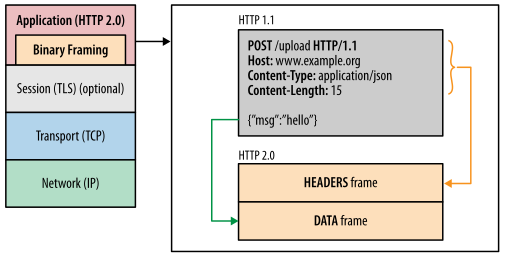
\includegraphics[scale=1.0]{\ImgPath/rys/ramka.png}
\end{center}
	\caption{Schemat ramki protokołu HTTP/2}
	\label{schematRamki}
\end{figure}
Jest to rozwiązanie dużo bardziej kompaktowe i łatwiejsze w implementacji, niż przesyłanie zwykłego tekstu.
Dzięki temu zabiegowi w ramach jednego połączenia TCP z serwerem może zostać utworzonych wiele dwukierunkowych strumieni danych przesyłających wiadomości HTTP.
Taka wiadomość to w rzeczywistości zapytanie od klienta lub odpowiedź serwera składające się z ramek.
Każda ramka natomiast musi przynajmniej posiadać nagłówek z informacją, do którego strumienia danych należy.
Kodowanie binarne nie ma wpływu na składnie zawartości ramki -- wszystkie nagłówki czy zapytania HTTP/1.1 pozostawiono bez zmian.

\section{Multiplexing}
\label{sectionMultiplexing}
W poprzedniej wersji protokołu, pomimo, że istniała możliwość przesyłania wielu zapytań w ramach jednego połączenia, nie można było wykonywać ich równolegle.
Każde zapytanie musiało być rozpatrywane i odesłane przez serwer do klienta zgodnie z kolejnością nadania, co powodowało efekt HOL (head-of-line blocking ODNOSNIK  DO JAKIEGOŚ ŹRÓDŁA?).
Aby wykonywać zapytania równolegle należało utworzyć kilka zapytań TCP, co obciąża serwer oraz jest czasochłonne.
Protokuł HTTP/2 umożlwia przesyłanie oraz odbieranie wielu wiadomości jednocześnie, co pokazuje schemat na rysunku \ref{schematMultiplexing}.
\begin{figure}[!htbp]
	\begin{center}
\centering
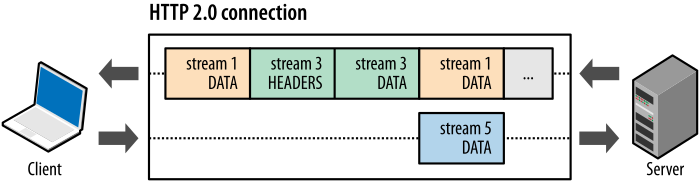
\includegraphics[scale=0.6]{\ImgPath/rys/multiplexing.png}
\end{center}
	\caption{Schemat wykorzystania multiplexingu w HTTP/2}
	\label{schematMultiplexing}
\end{figure}
Są one rozbijane na pojedyncze ramki, przesyłane, a następnie odczytywane i składane z powrotem w całość po stronie odbiorcy.
Dzięki temu nie jest już konieczne uciekanie się do takich zabiegów jak:
\begin{itemize}
	\item scalanie plików (WEBPACK),
	\item  wykorzystywanie spritów,
	\item domain sharding (DOCZYTAC).
\end{itemize}
To wszystko sprawia, że aplikacje stają się szybsze oraz prostsze.

\section{Prioretyzacja}

% wspomne o tym jesli zrobie testy

\section{Server push}
\label{sectionServerPush}

Wykorzystując protokół HTTP/1.1 nie mamy możliwości otrzymania zasobu, o który nie poprosiliśmy wysyłając zapytanie.
Powoduje to opóźnienia na przykład podczas ładowania strony internetowej.
Zanim otrzymamy skrypty czy arkusze styli, które wykorzystuje nasza strona musi ona o nie poprosić.
Zapytanie do serwera wysyłane jest gdy w kodzie pliku html napotkamy na taki kod (przykład z mojego projektu):
\begin{lstlisting}
<!-- CSS -->
<link rel="stylesheet"
	  href="libs/bootstrap/dist/css/bootstrap.min.css">
<link rel="stylesheet"
      href="libs/font-awesome/css/font-awesome.min.css">

<!-- JS -->
<script src="libs/angular/angular.min.js"></script>
\end{lstlisting}
Takie rozwiązanie, chociaż w wielu przypadkach jest pożądane, tutaj jedynie spowalnia działanie aplikacji.
Jeżeli mamy pewność, że użytkownik będzie potrzebował danych zasobów \ref{schematPush} możemy mu je od razu udostępnić, co zdecydowanie skraca czas ładowania aplikacji i dzięki temu unikam niechcianego efektu, gdy strona się załaduje, ale na przykład bez pliku zawierającego style, który jest dopiero przesyłany.
\begin{figure}[!htbp]
	\begin{center}
\centering
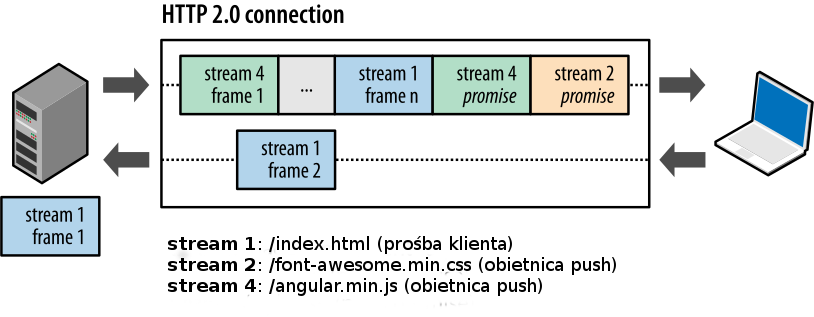
\includegraphics[scale=0.6]{\ImgPath/rys/push.png}
\end{center}
	\caption{Schemat Server push HTTP/2}
	\label{schematPush}
\end{figure}

%Podstawowy scenariusz, powszechny w literaturze na temat steganografii, odnosi 
%się do sytuacji opisanej w \cite{PrisonersProblem}. Dwóch więźniów (w naszym 
%przypadku Alicja(\tech{A}) i Bob(\tech{B})) zamknięci są w dwóch odrębnych 
%celach. 
%
%Przedstawioną tak sytuację pokazuje rysunek 
%\ref{schematKomunikacji}\footnote{sporządzony na podstawie 
%\cite{schematKomunikacjiPrzypis}, rysunek 1, strona 3}. \tech{A} próbuje 
%przesłać tajną informację \tech{E} do \tech{B}. Cała komunikacja odbywa się 
%przez kanał publiczny, kontrolowany przez \tech{W}. W celu ukrycia faktu 
%komunikacji \tech{A} stara się ukryć tajny przekaz w informacji \tech{C}. W celu 
%uzyskania skutecznej steganografii \tech{W} nie może rozróżnić informacji 
%poprawnej, nie zawierającej tajnych danych, od informacji \tech{S}, która 
%zawiera tajną informację. W celu dodatkowego zabezpieczenia przekazu, \tech{A} i 
%\tech{B} mogą korzystać z funkcji kryptograficznej zabezpieczającej przekazywane 
%informacje. Można tu wykorzystać metody kryptografii symetrycznej (ustalony 
%klucz kryptograficzny \tech{K}) lub niesymetrycznej (klucz publiczny 
%\tech{K}$_{pub}$ i klucz prywatny \tech{K}$_{pryw}$).


\section{Kompresja nagłówków}

\chapter{Budowa aplikacji}

\section{Struktura aplikacji}
\section{Aplikacja od strony serwera}

% ciekawe elementy
% opis bibliotek z github

\chapter{Testy}

\section{Chrome DevTools}

Do pomiaru prędkości oraz uzyskania innych ważnych informacji wykorzystałem narzędzie Chrome DevTools.
Opiszę tutaj po krótce co i jak mierzyłem za pomocą tego oprogramowania.

Po uruchomieniu konsoli przeglądarki przechodzimy do zakładki Network i naszym oczom ukazuje się okno jak na rysunku \ref{schematDevops}.

\begin{figure}[!htbp]
	\begin{center}
\centering
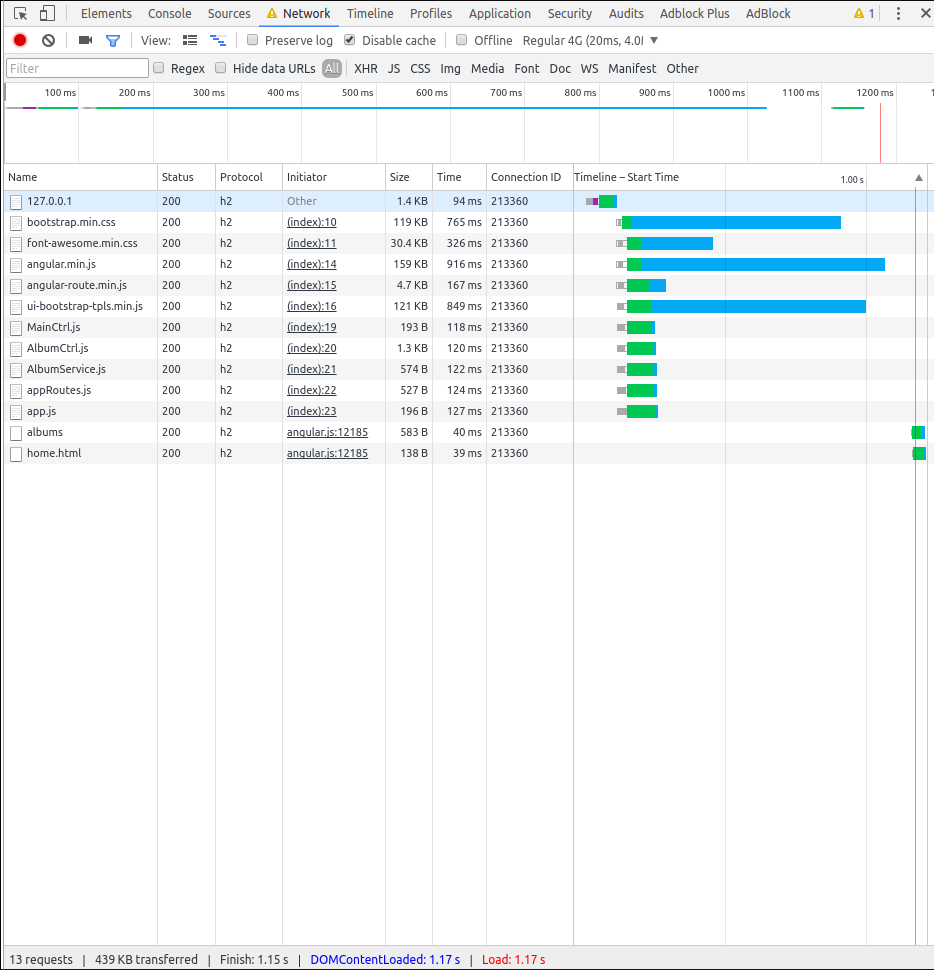
\includegraphics[scale=0.6]{\ImgPath/rys/devops.png}
\end{center}
	\caption{Wygląd okna Chrome DevTools}
	\label{schematDevops}
\end{figure}

Widoczne okno składa się z pięciu głównych elementów:
\begin{enumerate}
	\item paska kontroli -- umożliwia on między innymi edycję wyglądu panelu sieciowego,
	\item paska filtrów -- pozwala na stworzenie reguł i wybór tylko tych pakietów, które nas interesują,
	\item paska przeglądu -- ukazuje nam oś czasu, która daje nam obraz tego, jak przesyłane były pakiety danych,
	\item tabeli zapytań -- zawiera szczegółowe informacje na temat każdego zapytania
	\item podsumowania -- zawiera informacje o łącznej liczbie zapytań, przesłanych danych oraz czasie trwania.
\end{enumerate}

W moich badaniach najczęściej korzystałem z informacji zawartych w tabeli zapytań, a szczególnie z przedstawionej w niej osi czasu.
Po najechaniu kursorem na którykolwiek pasek na osi otrzymujemy szczegółowe informacje o czasie każdego z etapów zapytania jak na rysunku \ref{schematResourceTiming}.

\begin{figure}[!htbp]
	\begin{center}
\centering
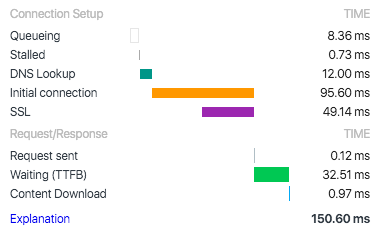
\includegraphics[scale=0.6]{\ImgPath/rys/resource-timing-data.png}
\end{center}
	\caption{Szczegółowe informacje na temat czasu zapytania}
	\label{schematResourceTiming}
\end{figure}

\section{Testy wstępne}

Przed przejściem do porównania prędkości działania obu wersji protokołu chciałem zaprezentować pierwsze efekty implementacji protokołu HTTP/2, które przedstawia rysunek \ref{schematWorkingExample}.

\begin{figure}[!htbp]
	\begin{center}
\centering
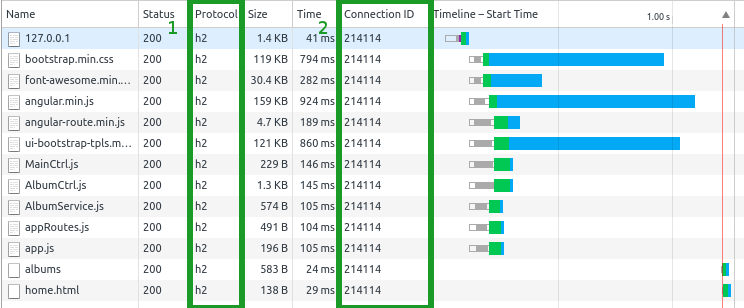
\includegraphics[scale=0.6]{\ImgPath/rys/workingExample.png}
\end{center}
	\caption{Dowód działania protokołu HTTP/2}
	\label{schematWorkingExample}
\end{figure}

Widzimy tutaj dwie rzeczy, które powinny nas zainteresować. W sekcji 'Protocol' oznaczonej na rysunku \ref{schematWorkingExample} numerem 1 widnieje napis h2 przy każdym zapytaniu.
Jest to informacja, że do komunikacji z serwerem wykorzystana została najnowsza wersja protokołu HTTP.
Dodatkowo w sekcji 'Connection ID' (na rysunku \ref{schematWorkingExample} jest to numer 2) widzimy, że wszystkie zapytania zostały wykonane z wykorzystaniem tego samego połączenia TCP.
Nie mogłoby to mieć miejsca, gdybyśmy wykorzystali HTTP/1.1, co pokazuje rysunek \ref{schematWorkingExampleH1}.

\begin{figure}[!htbp]
	\begin{center}
\centering
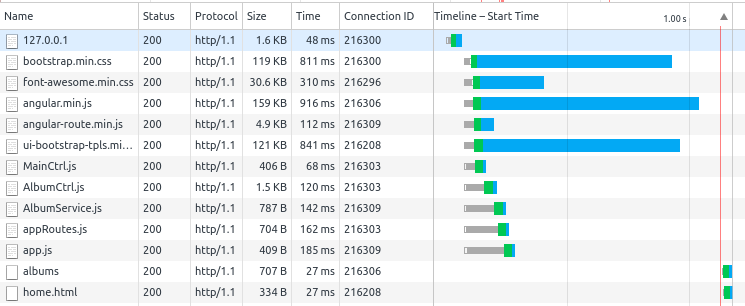
\includegraphics[scale=0.6]{\ImgPath/rys/workingExampleH1.png}
\end{center}
	\caption{Przykładowe linia czasu dla zapytań wykonanych w HTTP/1.1}
	\label{schematWorkingExampleH1}
\end{figure}

Na rysunku widzimy, że protokół z jakiego korzystamy to HTTP/1.1, a wszystkie zapytania, które są wykonywane równolegle przesyłane są w ramach różnych połączeń TCP.
Świadczą o tym wartości w kolumnie 'Connection ID'.

Jeszcze jedną ciekawą rzeczą są wielkości nagłówków.
Dzięki przejściu na kodowanie binarne nagłówki w protokole HTTP/2 są o wiele mniejsze niż te w jego starszym bracie.
W swojej pracy stworzyłem możliwość wysłania zapytania, które w odpowiedzi dostaje odpowiedź w postaci samego nagłówka.
Dzięki temu można porównać wielkość nagłówków HTTP na konkretnym przykładzie,
Wyniki przedstawiaja rysunki \ref{schematEmptyRes} i \ref{schematEmptyResH1}.

\begin{figure}[!htbp]
	\begin{center}
\centering
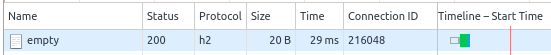
\includegraphics[scale=0.6]{\ImgPath/rys/emptyRes.png}
\end{center}
	\caption{Pusta odpowiedź w HTTP/2}
	\label{schematEmptyRes}
\end{figure}

\begin{figure}[!htbp]
	\begin{center}
\centering
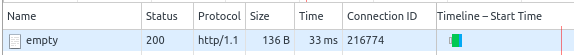
\includegraphics[scale=0.6]{\ImgPath/rys/emptyResH1.png}
\end{center}
	\caption{Pusta odpowiedź w HTTP/1.1}
	\label{schematEmptyResH1}
\end{figure}

Od razu widać, że nagłówki w najnowszej wersji protokołu uległy znacznej kompresji. 

%Przed przejściem do właściwych testów chciałem jeszcze zaznaczyć, że protokół HTTP/2 wymga wykorzystanie %bezpiecznego połączenia.
%Wygenerowałem własny certyfikat oraz potrzebne klucze i będę korzystał z bezpiecznego połączenia we wszystkich %pomiarach.

\section{Porównanie prędkości protokołu HTTP/2 i HTTP/1.1}

W ramach tego testu sprawdzałem prędkość ładowania wszystkich zasobów strony z wyłączonym CACHE przeglądarki oraz z ustawioną prędkością Regular 4G (20ms, 4.0 Mb/s, 3.0 Mb/s).
Dane z wykorzystaniem protokołu HTTP/1.1 są przesyłane za pomocą niezabezpieczonego połączenia.
HTTP/2 do utworzenia połączenia wymaga zabepieczenia SSL.

\begin{tabular}{c|c|c}
Próba & HTTP/1.1 & HTTP/2 \\ \hline
1 & 1.23s & 1.26s\\
2 & 1.49s & 1.12s\\
3 & 1.28s & 1.39s\\
4 & 1.20s & 1.09s\\
5 & 1.22s & 1.09s\\
6 & 1.25s & 1.26s\\
7 & 1.21s & 1.12s\\
8 & 1.25s & 1.11s\\
9 & 1.21s & 1.16s\\
10 & 1.26s & 1.10s\\ \hline
ŚREDNIA & 1.26s & 1.17s\\
\end{tabular}

Tabela ukazuje wyniki wykonanych pomiarów.
Jak widać protokół HTTP/2 przyśpiesza czas ładowania strony o około 15%.
W dużej mierze jest to czas zaoszczędzony na nawiązywanie nowych połączeń TCP.
Sporą oszczędność utrzymujemy też dzięki zmniejszeniu objętości nagłówków odpowiedzi.

Na rysunkach \ref{schematBasicTest} oraz \ref{schematBasicTestH1} widoczny jest przykładowy wynik testu.
W sekcji podsumowania widoczna jest całkowita objętość przesłanych danych. Są to odpowiednio 443 KB i439 KB dla protokołu HTTP/1.1 i HTTP/2,
Możemy też porównać objętości oraz czasy przesyłania poszczególnych plików.

\begin{figure}[!htbp]
	\begin{center}
\centering
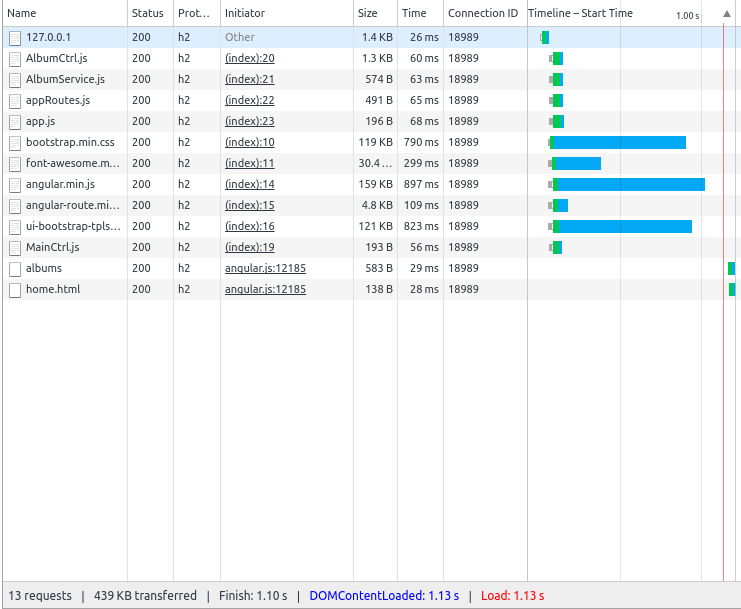
\includegraphics[scale=0.6]{\ImgPath/rys/basicTest.png}
\end{center}
	\caption{Test dla HTTP/2}
	\label{schematBasicTest}
\end{figure}

\begin{figure}[!htbp]
	\begin{center}
\centering
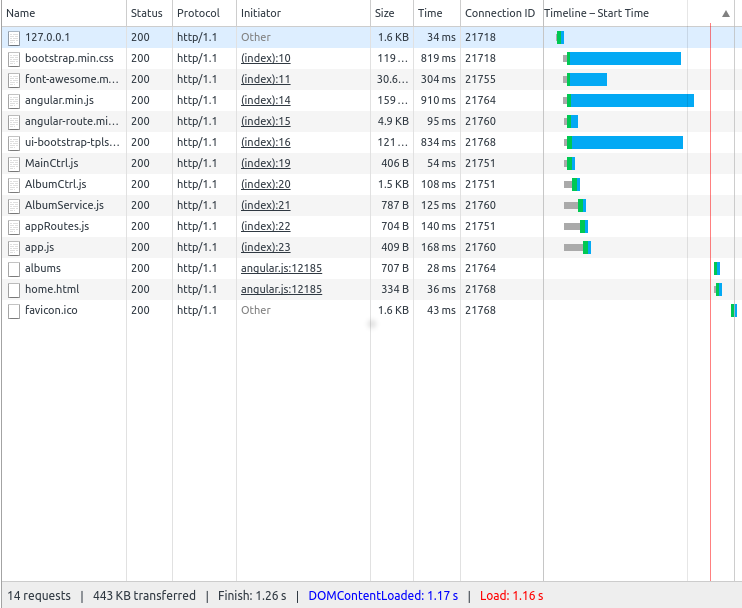
\includegraphics[scale=0.6]{\ImgPath/rys/basicTestH1.png}
\end{center}
	\caption{Test dla HTTP/1.1}
	\label{schematBasicTestH1}
\end{figure}

\section{Porównanie prędkości przy bezpiecznym połączeniu HTTP/1.1}

W tym teście dane przesyłane za pomocą protokołu HTTP/1.1 są zabepieczone SSL.

\begin{tabular}{c|c|c}
Próba & HTTP/1.1 & HTTP/2 \\ \hline
1 & 1.12s & 1.07s \\
2 & 1.20s & 1.09s \\
3 & 1.05s & 1.07s \\
4 & 1.12s & 1.09s \\
5 & 1.08s & 1.06s \\
6 & 1.10s & 1.11s \\
7 & 1.13s & 1.16s \\
8 & 1.09s & 1.15s \\
9 & 1.08s & 1.12s \\
10 & 1.11s & 1.10s\\ \hline
ŚREDNIA & 1.108s & 1.102s \\
\end{tabular}

Podczas tego testu otrzymałem zaskakujące wyniki.
Całkowity czas ładowania się zasobów strony dla protokołu HTTP/1.1 z wykorzystaniem SSL jest krótszy, niż przy nieszyfrowanym połączeniu.
Jest to zaskakujące, ponieważ szyfrowanie wymusza na nas podjęcie dodatkowych kroków na początku transmisji, które zabierają czas.


\section{Porównanie prędkości dla HTTP/1.1 z włączononym CACHE}

\begin{tabular}{c|c|c}
Próba & HTTP/1.1 & HTTP/2 \\ \hline
1 & & \\
2 & & \\
3 & & \\
4 & & \\
5 & & \\
6 & & \\
7 & & \\
8 & & \\
9 & & \\
10 & & \\ \hline
ŚREDNIA & & \\
\end{tabular}


\section{Porównanie prędkości przy wykorzystaniu Server Push}

\begin{tabular}{c|c|c}
Próba & HTTP/1.1 & HTTP/2 \\ \hline
1 & & \\
2 & & \\
3 & & \\
4 & & \\
5 & & \\
6 & & \\
7 & & \\
8 & & \\
9 & & \\
10 & & \\ \hline
ŚREDNIA & & \\
\end{tabular}


\chapter{Wnioski}

% co jeszcze moglem zrobic

%numery wygenerowane przy pomocy \tech{Shushi} nie byłyby rozróżnialne 
%od numerów wygenerowanych przez stos sieciowy systemu.
%
%\begin{tabular}{c|cc}
%pierwsza kolumna & druga & trzecia \\ \hline
%1 & 2 & 3 \\
%a & b & c \\
%\end{tabular} 
%
%\begin{equation}
% E = m c^2 \label{einstein}
%\end{equation}

%-----------------
% Dodatki 
%-----------------
%\appendix
%\chapter{}


\begin{thebibliography}{99}
\addcontentsline{toc}{chapter}{Bibliografia}
\bibitem{Stevens}{W. R. Stevens, G. R. Wright, ,,Biblia TCP/IP tom 1'', RM, 
1998.}
\bibitem{USDoD}{U. S. Department Of Defense, ,,Trusted Computer System 
Evaluation Criteria'', 1985.}
\bibitem{FirstCC}{B. W. Lampson, ,,A note on the confinment problem'', w ,,Proc. 
of the Communications of the ACM'', październik 1973, numer 16:10,\newline 
strony 613-615.} 
\bibitem{PrisonersProblem}{G. J. Simmons, ,,The prisoners' problem and the 
subliminal channel'', w ,,Advances in Cryptology: Proceedings of Crypto 83 (D. 
Chaum, ed.)'', strony 51-67, Plenum Press, 1984.}
\bibitem{Kerckhoff}{ A. Kerckhoffs, ,,La Cryptographie Militaire (Military 
Cryptography)'', J. Sciences Militaires, luty 1883.} 
\bibitem{Hanssen}{A. Havill, ,,The Spy Who Stayed Out In The Cold: The Secret 
Life of Double Agent Robert Hanssen'', St. Martin's Press, 2001.}
\bibitem{schematKomunikacjiPrzypis}{C.Cachin, ,,An Information-Theoretic Model 
for Steganography'', w ,,Information and Computation'', 4 marzec 2004.}
\bibitem{SweetyPresentation}{S.Chauhan, ,,Embedding Covert Channels into 
TCP/IP'', 7th Information Hiding Workshop, czerwiec 2005.}
\bibitem{RFC793}{Information Sciences Institute, University of Southern 
California, ,,Transmission Control Protocol'', RFC793, wrzesień 1981.}
\bibitem{RFC1323}{V. Jacobson, R. Braden, D. Borman, ,,TCP extensions for high 
performance'', RFC1323, maj 1992.}
\bibitem{RFC1948}{S. Bellovin, ,,Defending against sequence number attacks.'', 
RFC1948, IETF, 1996.}
\bibitem{RFC2960}{R. Stewart, Q. Xie, K. Morneault, C. Sharp, H. Schwarzbauer, 
T. Taylor, I. Rytina, M. Kalla, L. Zhang, V. Paxson, „Stream Control 
Transmission Protocol”, RFC2960, Network Working Group, październik 2000.}
\bibitem{Rowland}{C. H. Rowland, ,,Covert Channels in the TCP/IP Protocol 
Suite'', First Monday, 1997. \newline 
\url{http://www.firstmonday.dk/issues/issue2\_5/rowland/}}
\bibitem{LOKI}{Alhambra, daemon9, ,,Project Loki: ICMP Tunneling'', Phrack 
Magazine, Issue 49. \url{http://phrack.org}}
\bibitem{LOKI2}{daemon9, ,,LOKI2'', Phrack Magazine, Issue 51. 
\url{http://phrack.org}}
\bibitem{RWWWS}{van Hauser, Reverse WWW Shell,  THC, The Hacker's 
Choice.\newline \url{www.thc.org}}
\bibitem{CCdetectionSVM}{T. Sohn, J. Seo, J. Moon, ,,A Study on the Covert 
Channel Detection of TCP/IP Header Using Support Vector Machine'', Volume 2836 
of Lecture Notes in Computer Science., Springer-Verlag (2003) 313-324.}
\bibitem{LOKIdetectionSVM}{T. Sohn, T. Noh, J. Moon, ,,Support Vector Machine 
Based ICMP Covert Channel Attack Detection'', Volume 2836 of Lecture Notes in 
Computer Science., Springer-Verlag, 2003, strony 461-464.}
\bibitem{devcc}{J. Giffin, R. Greenstadt, P. Litwack, R. Tibbetts, ,,Covert 
messaging in TCP'', w Dingledine, Privacy Enhancing Technologies. Volume 2482 of 
Lecture Notes in Computer Science., Springer-Verlag (2002) 194-208. 
\url{http://www.mit.edu/\textasciitilde gif/covert-channel/}}
\bibitem{ActiveWardens}{G. Fisk, M. Fisk, Ch. Papadopoulos, J. Neil, 
,,Eliminating Steganography in Internet Traffic with Active Wardens'', 5th 
International Workshop on Information Hiding, październik 2002.} 
\bibitem{JR}{J. Rutkowska, ,,The Implementation of Passive Covert Channels in 
Linux Kernel'', Chaos Communication Congress, grudzień 2004.}
\bibitem{LinuxNetwork}{Ch. Benvenuti, ,,Understanding Linux Network Internals'', 
O'Reilly,\newline grudzień 2005.}
\bibitem{p55}{kossak, ,,Building Into The Linux Network Layer'', Phrack 
Magazine, Issue 55. \url{http://phrack.org}}
\bibitem{ML}{Steven J.Murdoch and Stephen Lewis, ,,Embedding Covert Channels 
into TCP/IP'', University of Cambridge, Computer Laboratory,\newline 29 lipec 
2005.}
\bibitem{NvsNN}{Eugene Tumoian, Maxim Anikeev, ,,Detecting NUSHU Covert Channels 
Using Neural Networks'', Taganrog State University of Radio Engineering, 
Department of Information Security.}
\bibitem{p58}{mayhem, ,,IA32 Advanced Function Hooking'', Phrack 
Magazine,\newline Issue 58. \url{http://phrack.org}}
\bibitem{p61}{bioforge, ,,Hacking the Linux Kernel Network Stack'', Phrack 
Magazine, Issue 61. \url{http://phrack.org}}
\bibitem{kernelMEM}{Robert Love, ,,Kernel Korner - Allocating Memory in the 
Kernel'',\newline 1 grudzień 2003.}

\end{thebibliography}

%\zakonczenie  % wklejenie recenzji i opinii

\end{document}
%+++ END +++
